\chapter{Cell assemblies analysis}
\label{chap:AssemblyAnalysis}
In this chapter we present the assembly analysis conducted on the data set presented in \autoref{chap:Dataset}, using the cell assembly algorithm and the single units classification respectively presented in \autoref{chap:AssemblyMethod} and \autoref{chap:UnitsAnalysis}.
The algorithm is free to detect any spike pattern coordination at any time scale.
Thus, applying the cell-assembly algorithm we were able to detect synchronous ($lag=0$) and asynchronous ($lag\neq 0$) cell assemblies at arbitrary time scale ($\Delta$). The time scales are explored running over different bin sizes of assembly-detection, and the lag, that is one outcome of the cell assembly algorithm, is the temporal distance in activation between units in assembly.
Since we were interested in cross areal interactions an directionality between Ventral Striatum and Ventral Tegmental Area, in this work we focus on inter-regional assembly-pairs. Inter-regional assembly-pairs are assemblies formed by two neurons, of which one neuron is in Ventral Striatum and one neuron is in Ventral Tegmental area. This is  an intuitive way to study the directionality between two regions: at pairs-level in fact, the lag in activation between units in assembly indicates the lag in activation between the two regions of concern. In our nomenclature a positive lag ($lag>0$) means that the VS unit is preceding in activation the VTA unit: VS is leading and VTA is following; while a negative lag ($lag<0$) means that the VTA unit is preceding the activation of the VS unit: we can say that VTA is leading and VS is following. 

\section{Cell types occurrence}
Using the units classification, inter-regional pairs were classified according to underlying cell types. 
\begin{figure}[H]
    \centering
    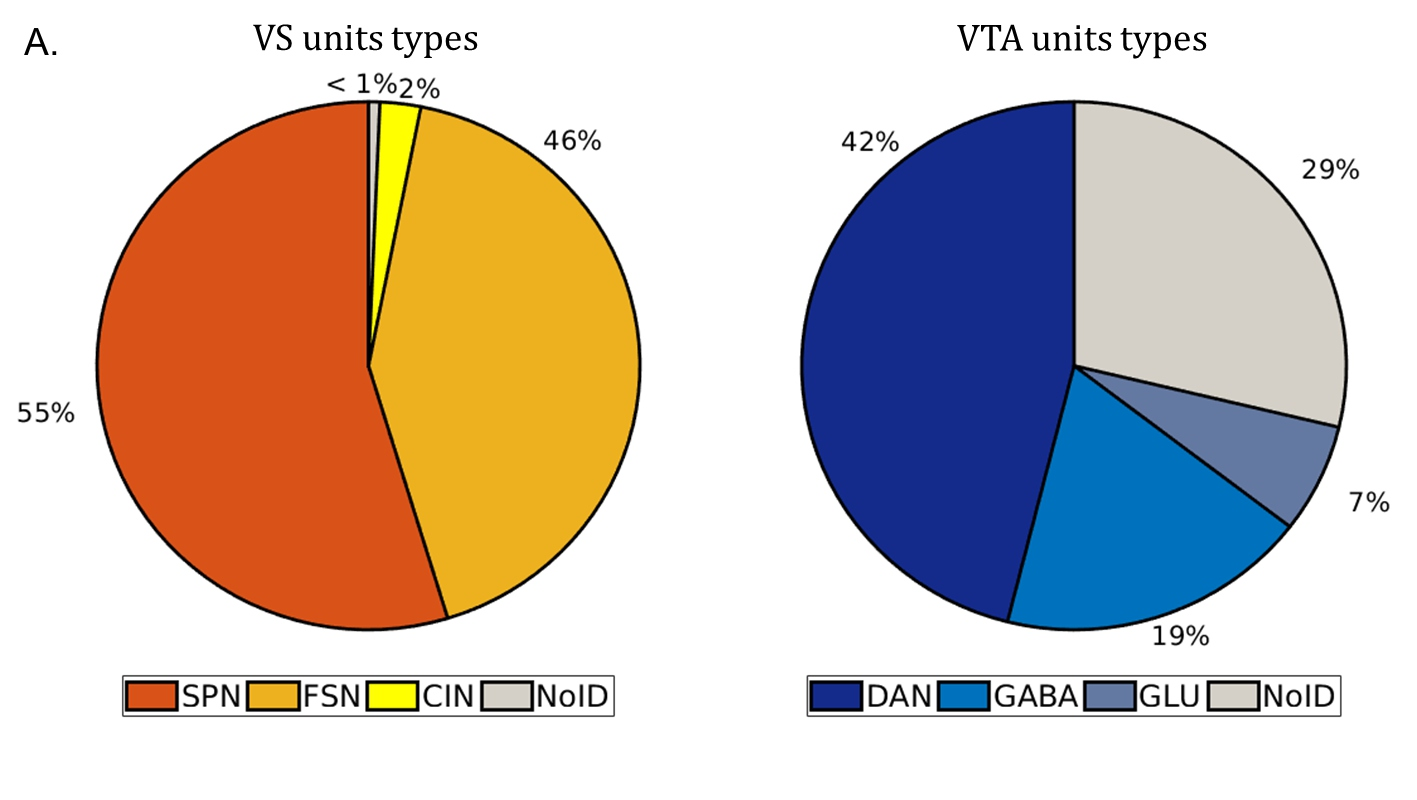
\includegraphics[scale=0.35]{figures/PieRegions1.pdf}
    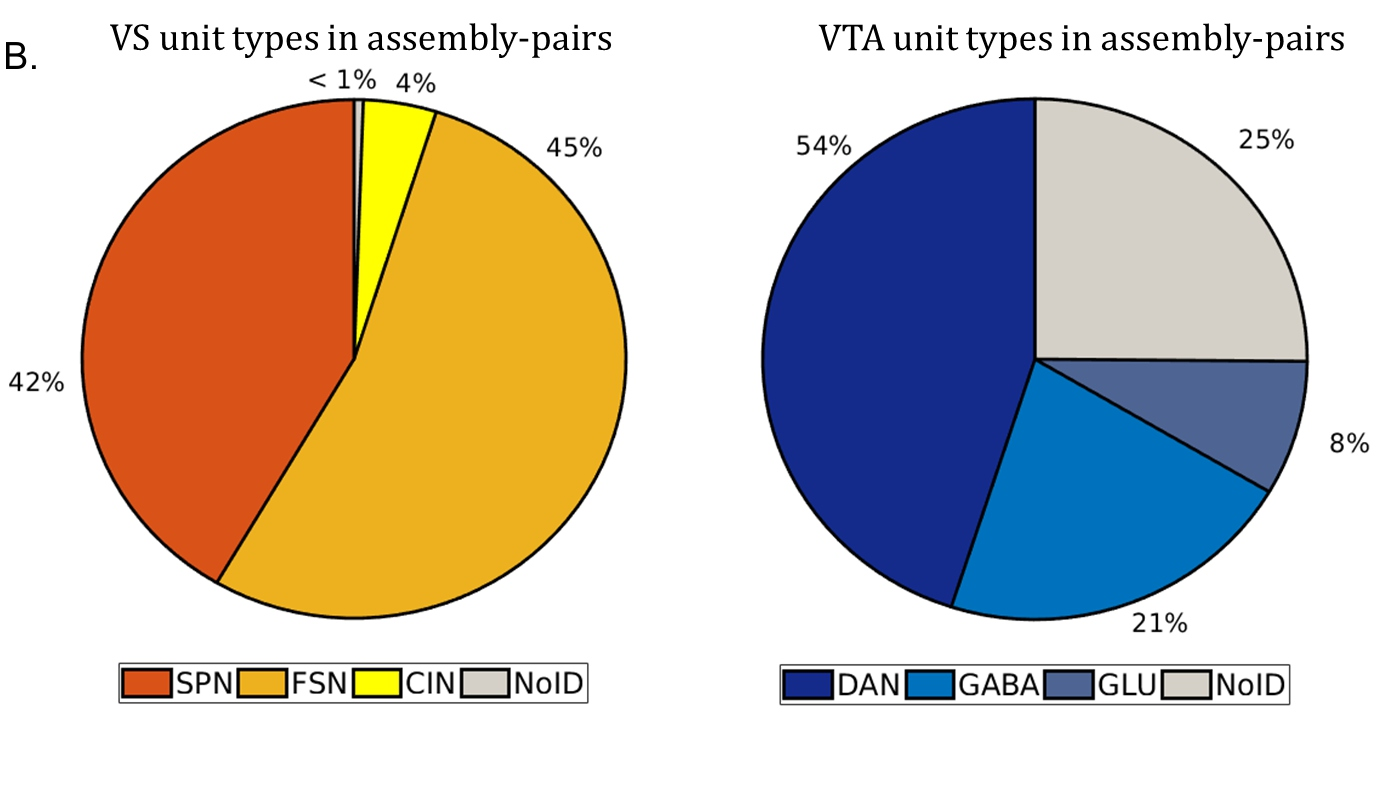
\includegraphics[scale=0.35]{figures/PieAsNotAs.pdf}
    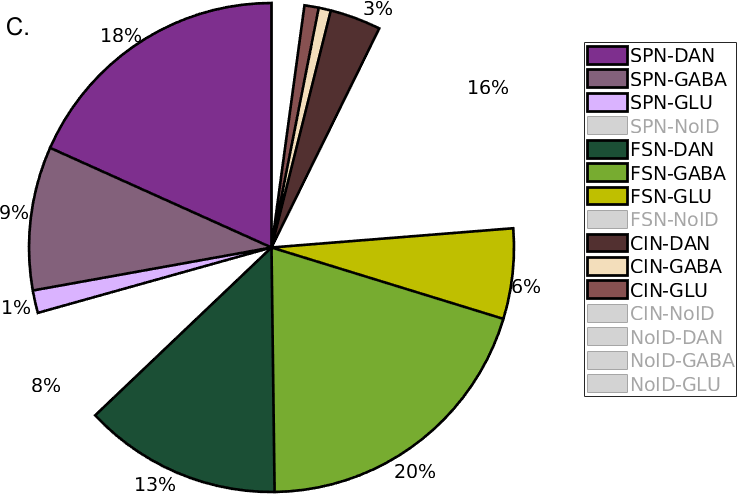
\includegraphics[scale=0.35]{figures/PieAssembliesTot1.png}
    \caption{(Top) Occurrence of classified and not classified units in VS and VTA. (Middle) Occurrence of classified and not classified units of VS and VTA in inter-regional assembly-pairs. In VS, FSN occur in inter-regional pairs more often than SPN, even though FSN are less represented than SPN.(Bottom)Pie charts of assemblies types. Not indicated percentage are $<1\%$. Missing pieces of cake indicates pairs that include not classified units. The first four more represented inter-regional pairs including only classified units are pairs between fast spiking and gabaergic neurons ($20\%$), striatal projection neurons and dopaminergic neurons ($18\%$), fast spiking and dopaminergic units ($13\%$) and striatal projecton and gabaergic units ($9\%$). }
    \label{fig:PieAssembliesTot}
\end{figure}
Classified and not classified units of VS and VTA occurred in assemblies as shown in fig. (\ref{fig:PieAssembliesTot} (top)). The inter-regional pairs formed by those units occurred as is shown in pie-chart in fig. (\ref{fig:PieAssembliesTot} (bottom)). We can see that, selecting only classified units, four assemblies types occurs more often than other, they are pairs formed by fast spiking and gabaergic neurons ($20\%$), striatal projection neurons and dopaminergic neurons ($18\%$), fast spiking and dopaminergic units ($13\%$) and striatal projecton and gabaergic units ($9\%$). Occurrence of classified and not classified units of VS and VTA in inter-regional assembly-pairs. In VS, fast spiking neurons occur in inter-regional pairs more often than striatal projection neurons, even though FSN are less represented than SPN. We hypotesize inter-regional pairs formation depends on the underlying unit-types, to verify this hypothesis we conducted for each of the two regions a Pearson$'$s $\chi^2$ test. Of the classified unit types, only the more recurrent were tested namely striatal projecton neurons and fast spiking neurons in VS, and dopaminergic and gabaergic units in VTA. This choice was made because cohlinergic interneuorns and glutamertegic units are poorly represented in this data-set, and in the entire work we focus on the four more represented neuron types and pairs between those units. Each unit is or not part of an inter-regional pair, in this way the contingencies tables (\ref{tab:chi2_asnotasVS} \ref{tab:chi2_asnotasVTA}) were created. For each test we choose the $\alpha$ significance level at $0.05$, unless differently specified.
\begin{table}[H]
    %\centering
\begin{tabular}{ |p{3cm}|p{3cm}|p{3cm}| }
 \hline
 \multicolumn{3}{|c|}{Pearson$'$s $\chi^2$ test VS unit type and inter-regional pair relationship} \\
 \hline
 & In pairs & Not in pairs\\
 \hline
 SPN & 153 (197.64) & 253 (208.36) \\
 \hline
 FSN & \textbf{197 (156.36)} & 116 (164.64)\\
 \hline
 \multicolumn{3}{|c|}{$\chi^2$ statistic  45.13}\\
 \multicolumn{3}{|c|}{p-value = $1.8\times10^{-11}$}\\
 \hline
 \multicolumn{3}{|c|}{$\chi^2$ statistic Yates correction 44.12}\\
 \multicolumn{3}{|c|}{p-value = $3.1\times10^{-11}$}\\
 \hline
\end{tabular}
\caption{Pearson$'$s $\chi^2$ contigency table with $\chi^2$ value and p-value. Unit types and inter-regional pairs formation are correlated in Ventral Striatum.}
\label{tab:chi2_asnotasVS}
\end{table}
\begin{table}[H]
    %\centering
\begin{tabular}{ |p{3cm}|p{3cm}|p{3cm}| }
 \hline
 \multicolumn{3}{|c|}{Pearson$'$s $\chi^2$ test VTA unit type and inter-regional pair relationship} \\
 \hline
 & In pairs & Not in pairs\\
 \hline
 DAN & 86 (90.604) & 31 (26.40) \\
 \hline
 GABA & 41 (36.40) & 6 (10.60)\\
 \hline
 \multicolumn{3}{|c|}{$\chi^2$ statistic  3.62}\\
 \multicolumn{3}{|c|}{p-value = 0.057}\\
 \hline
\end{tabular}
\caption{Pearson$'$s $\chi^2$ contigency table with $\chi^2$ value and p-value. Unit types and inter-regional pairs formation are not correlated in Ventral Tegmental Area.}
\label{tab:chi2_asnotasVTA}
\end{table}
A relationship between unit types and inter-regional pairs formation was found only in Ventral Striatum. In VS the $\chi^2$ statistic value is 45.13 (44.12 using Yates correction), that gives a p-value of $1.8\times10^{-11}$ ($3.1\times10^{-11}$), largely significant at $\alpha$ level. The result confirms our hypothesis that neuron-type in VS effects the formation of inter-regional assembly-pairs. The same test was conducted in VTA, with a resulting $\chi^2$ statistic of $3.62$ and a p-value of $0.057$, not significant at $\alpha = 0.05$ level. We can conclude then that in VTA different neuron-types have the same probability to form inter-regional pairs.
To see whether assembly types occur by chance or there is a relationship between the unit type activated in one region and the resulting assembly pairs, again Pearson's $\chi^2$ test were conducted. For each unit type we count  Specifically, given the pairs types occurrence, we hypothesize a preference by fast spiking neurons for gabaergic neurons (and/or vice-versa) and a preference by striatal projecton neurons for dopaminergic neurons (and/or vice-versa). The $\chi^2$ test were performed on the directional pairs ($lag\neq0$) and separately on $vs\rightarrow vta$ ($lag>0$) and $vs \leftarrow vta$ ($lag<0$). In both cases, the $\chi^2$ test revealed a dependence between the unit-type and the resulting inter-regional pairs. The p-values of $\chi^2$ test were significant at the confidence level $\alpha = 0.05$. In direction $vs\rightarrow vta$ $p=2\times10^{-4}$ ($p=4\times10^{-4}$ using Yates correction), in direction $vs \leftarrow vta$: $p=9\times10^{-3}$ ($p=0.017$ using Yates correction). In tables (\ref{tab:chisquare_vsvta} and \ref{tab:chisquare_vtavs}) are shown the contingency tables of the $\chi^2$ tests for the two directionalities. In rows the activated cell types of the leading region, in columns the coupled selected cell types of the follower region. In the tables are shown the number of pairs between the two cell-types and in brackets $()$ the expected values. Both in $vs\rightarrow vta$ and in $vs\leftarrow vta$ directionality the real value of couples $SPN+DAN$ and $FSN+GABA$ exceed the expected value as we hypothesized. The preference does not depend on directionality.
\begin{table}[H]
    %\centering
\begin{tabular}{ |p{3cm}|p{3cm}|p{3cm}| }
 \hline
 \multicolumn{3}{|c|}{Pearson$'$s $\chi^2$ test ($vs \rightarrow vta$)} \\
 \hline
 & DAN pairs & GABA pairs\\
 \hline
 SPN & 76 (63.77) & 35 (47.23) \\
 \hline
 FSN & 32 (44.23) & 45 (32.77)\\
 \hline
 \multicolumn{3}{|c|}{$\chi^2$ statistic  13.47}\\
 \multicolumn{3}{|c|}{p-value = $2\times10^{-4}$}\\
 \hline
 \multicolumn{3}{|c|}{$\chi^2$ statistic Yates correction 12.39}\\
 \multicolumn{3}{|c|}{p-value = $4\times10^{-4}$}\\
 \hline
\end{tabular}
\caption{Pearson$'$s $\chi^{2}$ test contingency table. We test the dependency between the neuron type in VS and the neuron type in VTA with which the pair is formed, for pairs with specific directionality $vs \rightarrow vta$. The $\chi^2$ test show a dependency among variables, meaning that resulting pair depends on the neuron types involved.}
\label{tab:chisquare_vsvta}
\end{table}

\begin{table}[H]
\begin{tabular}{ |p{3cm}|p{3cm}|p{3cm}| }
 \hline
 \multicolumn{3}{|c|}{Pearson$'$s $\chi^2$ test ($vs \leftarrow vta$)} \\
 \hline
 & SPN pairs & FSN pairs\\
 \hline
 DAN & 18 (12.06) & 29 (34.94) \\
 \hline
 GABA & 11 (16.94) & 55 (49.06)\\
 \hline
 \multicolumn{3}{|c|}{$\chi^2$ statistic  6.73}\\
 \multicolumn{3}{|c|}{p-value = 0.009}\\
 \hline
 \multicolumn{3}{|c|}{$\chi^2$ statistic Yates correction 5.65}\\
 \multicolumn{3}{|c|}{p-value = 0.017}\\
 \hline
\end{tabular}
\caption{Pearson$'$s $\chi^{2}$ test contingency table. We test the dependency between the neuron type in VTA and the neuron type in VS with which the pair is formed, for pairs with specific directionality $vs \leftarrow vta$. The $\chi^2$ test show a dependency among variables, meaning that resulting pair depends on the neuron types involved.}
\label{tab:chisquare_vtavs}
\end{table}
\section{Cross areal interactions time scales}
In this chapter a study on time scales involved in cross-areal interactions is presented. From the bimodal temporal scale ($\Delta$) distribution of cross-areal interaction emerges a segregation in two time scales for cross-areal interaction (figure (\ref{fig:BinDistr})).
\begin{figure}[H]
%\centering
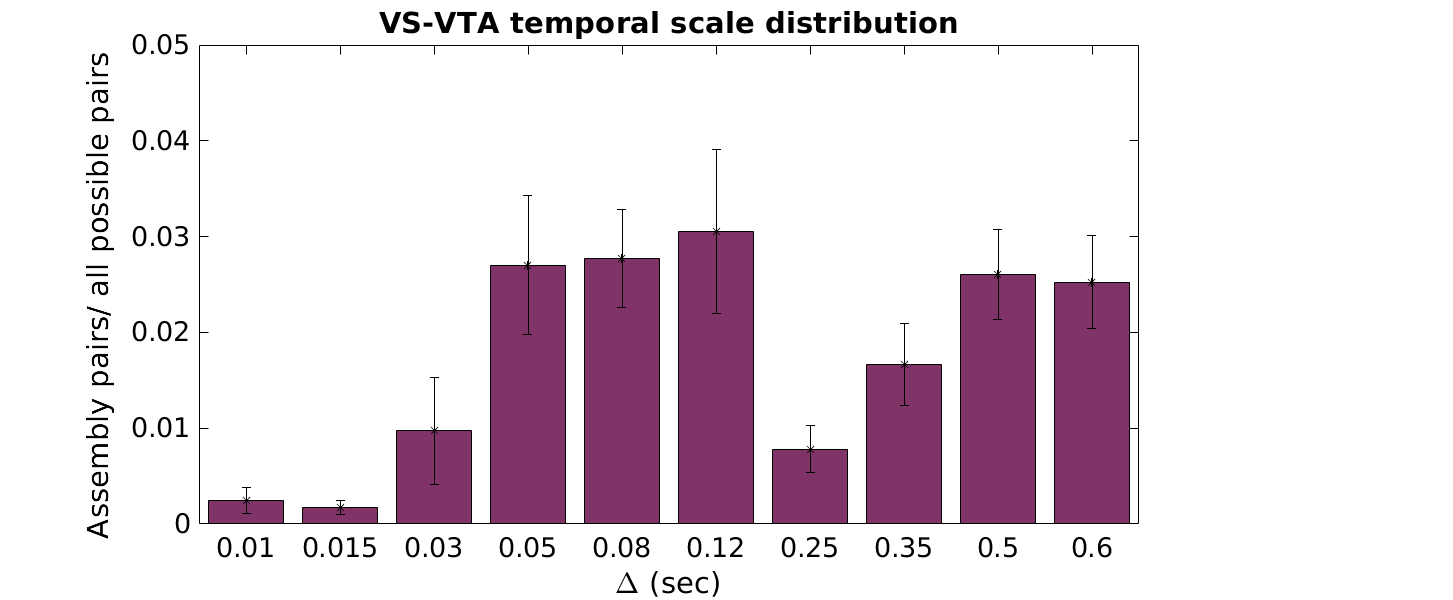
\includegraphics[scale=0.45]{figures/VS_VTA_Short1.png}
\caption{Bin distribution for inter-regional pairs. VS-VTA pairs show a bimodal distribution, meaning two temporal scale involved in inter-regional activation patterns.%B) VS-VS pairs bin distribution presents a peak at 50 $ms$, specifically in this region the pairs MSN-FSI high show an highly peaked distribution, almost centered at the peak of 50 $ms$, plot (B.2), while in MSN-FSI low distribution, albeit the peak is still at 50 $ms$, is evident the predominance of very precise time scales, including bins from 10 $ms$ to 50 $ms$, with respect to the larger time scale plot (B.1).
}
\label{fig:BinDistr}
\end{figure}
\begin{figure}[H]
%\centering
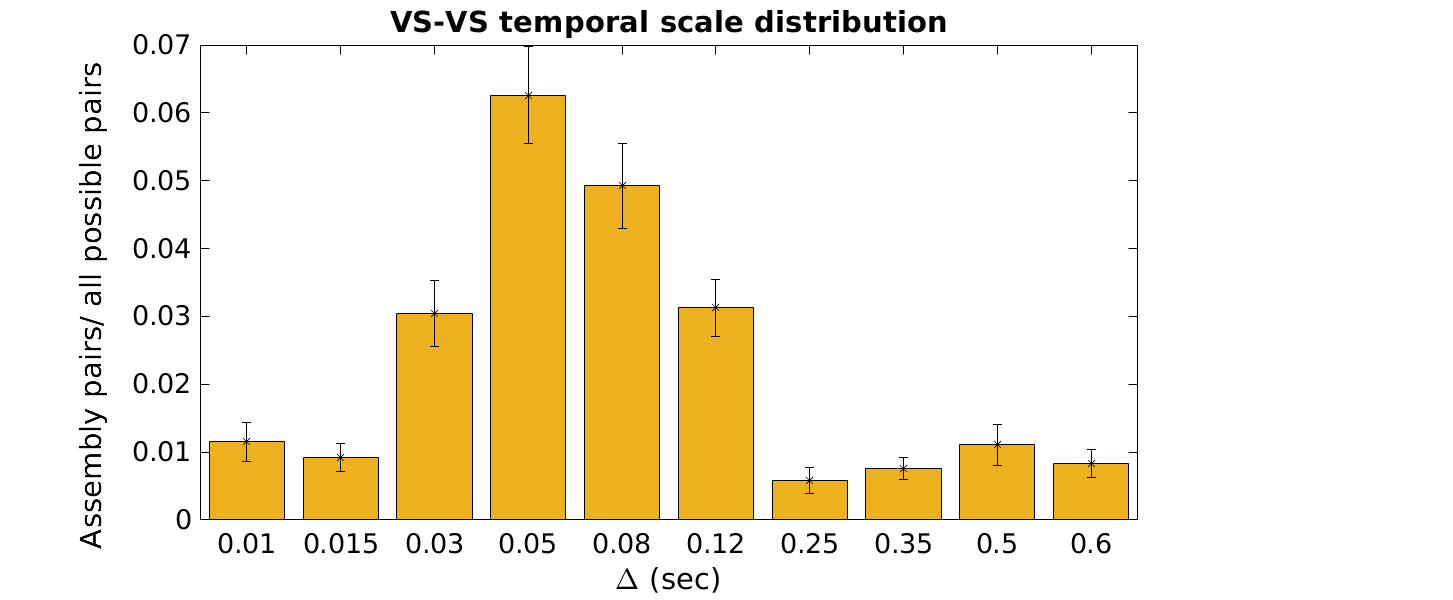
\includegraphics[scale=0.45]{figures/VS_VS_S.png}
\caption{VS-VS pairs bin distribution presents a peak at 50 $ms$}
\label{fig:BinDistr}
\end{figure}
\begin{figure}[H]
%\centering
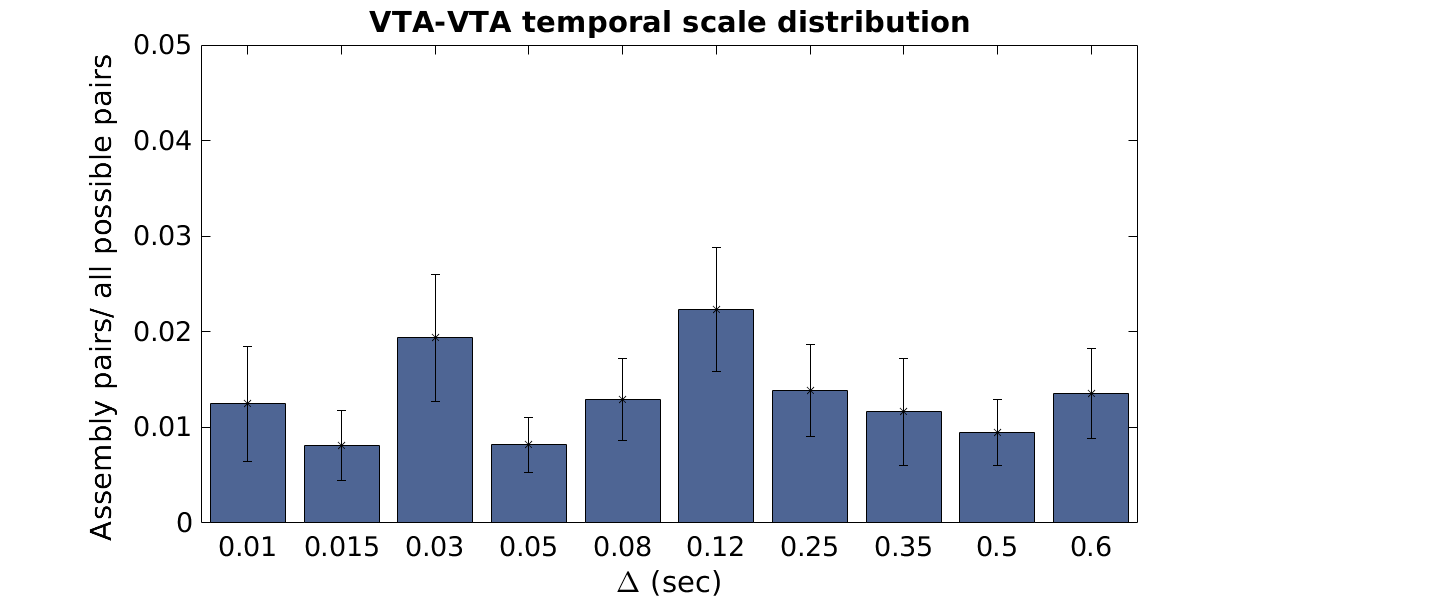
\includegraphics[scale=0.45]{figures/VTA_VTA_S.png}
\caption{VTA-VTA temporal scale distribution does not present any peak.}
\label{fig:BinDistr}
\end{figure}
This segregation is typical of inter-regional pairs, in fact a comparison with intra-regional pairs in Ventral Striatum and Ventral Tegmantal area show interesting differences.
While we observed assemblies of temporal precision at the scale of few tens of milliseconds only within either VS or VTA, assemblies of lower temporal precision were detected across VS-VTA units. The temporal precision of this last group displayed a bimodal distribution with peaks around $80$ milliseconds and one $1.6$ second, revealing the presence of two time scales, the first, preciser, ranged from 10 $ms$ to 250 $ms$, and the second including broader bin sizes. Intra-regional VTA-VTA pairs instead don't present any peak in time scales distribution. Intra-regional VS-VS bin size distribution is peaked around 50 $ms$. In VS we noticed differences between SPN and high-firing-rate SPN pairs and SPN and low-firing-rate FSN bin size distributions: specifically the firsts show higher temporal precision than the latter. {\color{red}{Include Figure of SPN -FSN and caption of bin size distribution}}.
\section{Directionality} 
The considerations above on the time scales distribution led us to study separately lag distribution of VS-VTA pairs detected in preciser and broader temporal scales highlighted from bin sizes distribution. We divided then these two assemblies population for the further study of directionality.
Interestingly lag distribution of precise and broad time scales are both asymmetric, indicating that the VS activation leads the activation of the VTA neuron (fig. \ref{fig:LagInSecAll}). The two distribution show however remarkable differences: broader time scales pairs distribution is fat-long tailed, whereas precise time scales lag distribution has thin tails.
We focused the study on the more precise temporal scale, in such a way that temporal scale interactions were separated to typical task-related times-scales, such as the length of the odor duration that cover typically $1.5 sec$.  we observed that specifically, the directional assemblies were composed of striatal and pallidal projection neurons leading dopaminergic VTA neurons (MSN and Type I pairs). Importantly, inter unit activation lags of assemblies containing pallidal neurons (FSI) were shorter than those containing striatal projection neurons (MSN), compatibly with assumed connectivity.
\begin{figure}[H]
\centering
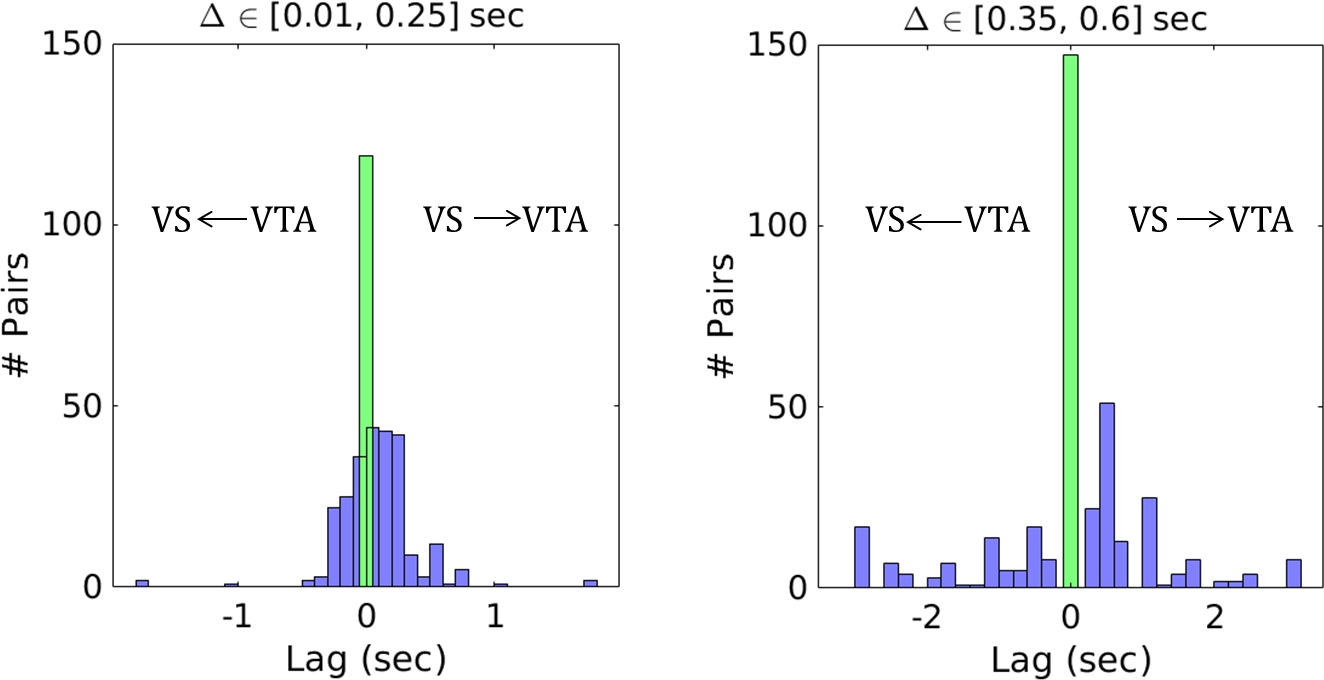
\includegraphics[scale=0.6]{figures/LagGeneral1.pdf}
\caption{Lag distribution for VS-VTA pairs in seconds. In green the synchronous pairs. On the left, lag distribution for pairs detected in preciser time scales. Slight distribution asymmetry indicates directionality in the direction of $lag > 0$, meaning a predominance of pairs in which VS leads VTA. On the right, the lag distribution for pairs detected in the broader time scale.}
\label{fig:LagInSecAll}
\end{figure}

\begin{figure}[H]
\centering
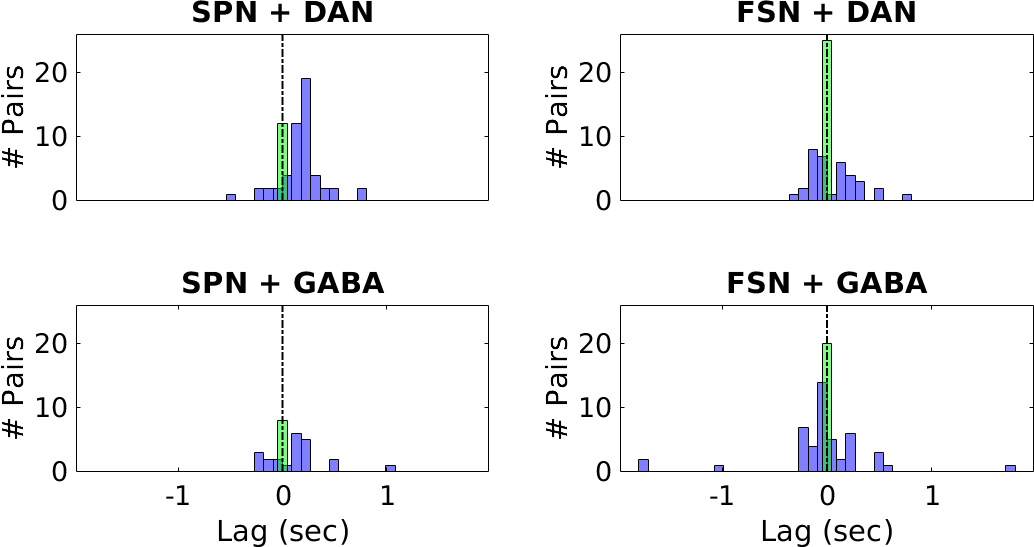
\includegraphics[scale=0.4]{figures/LagSec4Typo3VS.png}
%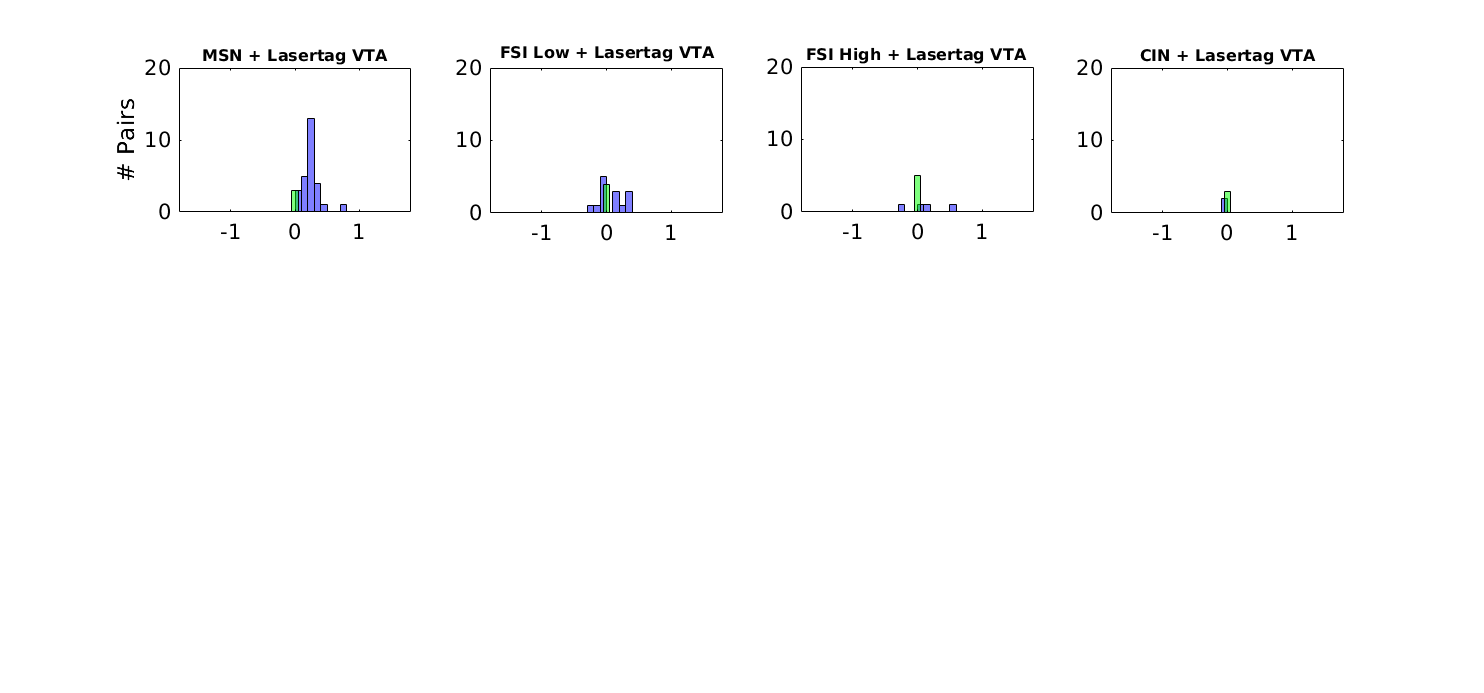
\includegraphics[scale=0.4]{figures/OnlyLaserOriz.png}
\caption{blabla}
\label{fig:LagInSecAll}
\end{figure}
In fig. (\ref{fig:directional_assembly}) a directional assembly. On top is shown mean and standard deviation of the assembly's activity for paired (grey line) and unpaired odor trials (purple line) in the original phase. On bottom raster plot and firing rate (mean and standard deviation) of units in assembly. x-axis origin correspond to the odor onset, while the red line marks the end of the stimulus duration. The examined assembly has a positive lag, that means VS preceding in activity VTA, from neuronal activity we can see in fact the VS unit activate before than the VTA unit. The assembly was detected with a bin size of $0.25 sec$, meaning that we are in the small temporal scale domain, in which the directionality clearly emerged. From the raster plot is evident that this kind of activation was persistent in each trial, in fact that assembly showed a significant task related activity after the stimulus. In term of assembly coding capability it is interesting to note the different activation for paired odor trials and unpaired odor trials, revealing the odor discrimination capability of the assembly. 
\begin{figure}
    \centering
    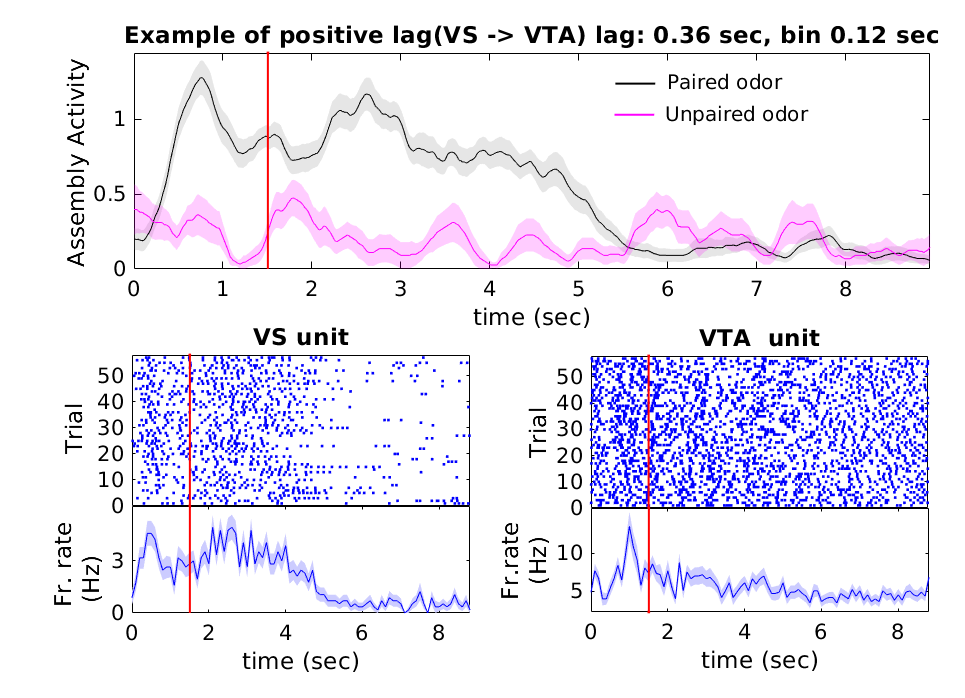
\includegraphics[scale=0.4]{figures/1_21Lastrev1Pru_An4Poster2.png}
    \caption{Directional assembly. On top mean and standard deviation of the assembly's activity for paired (grey) and unpaired odor trials (purple) in the original phase. On bottom raster plot and firing rate (mean and standard deviation) of units in assembly. x-axis origin correspond to the odor onset, while the red line marks the end of the stimulus duration. The examined assembly has a positive lag, that means VS preceding in activity VTA, from neuronal activity we can see in fact the VS unit activate before than the VTA unit.}
    \label{fig:directional_assembly}
\end{figure}
Bin width and lags analysis reveals time scale segregation, that can reveal in turn different assembly-activation patterns. In fig.(\ref{fig:AsActBinLag}) heat maps of assembly activity, detected in a particular paradigm, show differences in activation patterns among different bin width and lag. %% In the paradigm in examination animals were well-trained, it was the third time that the same couple of odor were presented with the same stimulus duration length.
\begin{figure}
    \centering
    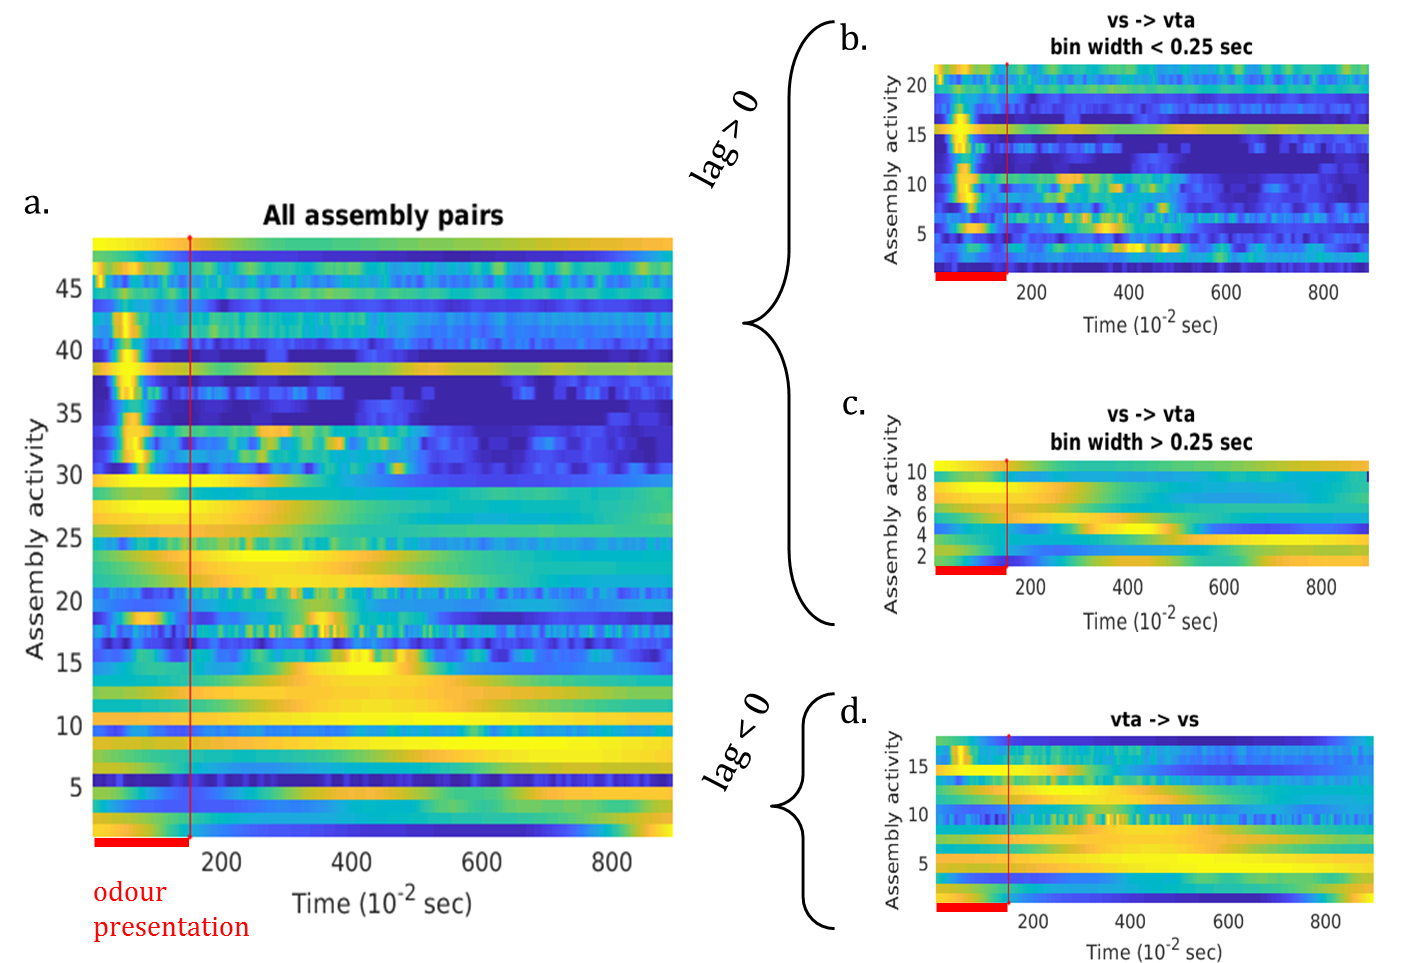
\includegraphics[scale=0.45]{figures/AsActPerBinLag1.png}
    \caption{Assembly-activation patterns given time bins and lags. In a.) totality of assemblies of one experimental paradigm, b,c,d. assemblies of same paradigm of a. selected for bin size ($\Delta$) and lag, $\Delta < 0.25 s$ and $lag > 0$ (b.), $\Delta > 0.25 s$ and $lag > 0$ (c.), $lag < 0$ (d.)}
    \label{fig:AsActBinLag}
\end{figure}
{\color{red}Include fig with all reversal paradigm and see which differences can be mentioned!!!}
\section{Conclusion}
From the inter-regional time precision distribution (bin size $\Delta$) we deduced that VS-VTA interactions are two time scales interactions. Looking at the assembly activity patterns we observed a dissection between the more precise time scale and the broader time scale inter-regional pairs. 
With the lags between units activation we have distinguished three types of assemblies: synchronous, positive directional and negative directional assemblies. From lag distributions one deduces that precise and broad time scale pairs show directionality in the direction of VS leading VTA.
Directional assemblies are formed by Striatal Projection Neurons and Dopaminergic Neurons.
Does directional assemblies show a different coding features with respect to other assemblies types?
To address this question we first investigate the assemblies task related pattern.
  
 \section{Differences among assemblies types}
 
 %%First difference between original and reversal phase is number of assemblies responding during the post-stimulus interval, this number decrease for all the typologies involved during hit trials (as shown in fig. (\ref{fig:histo_taskrel})), in according to the intuition, in reversal phase in fact, when the animals became more expert, neuronal response tend to be shifted closer to the reward delivery. This effect can be seen in fig. (\ref{fig:NeusInAsse}) where activity and raster plots of two units in a pair are shown. Looking at the raster plots, a shift in correspondence to the phase-switch is evident in both units.
 %\begin{figure}
  %   \centering
  %   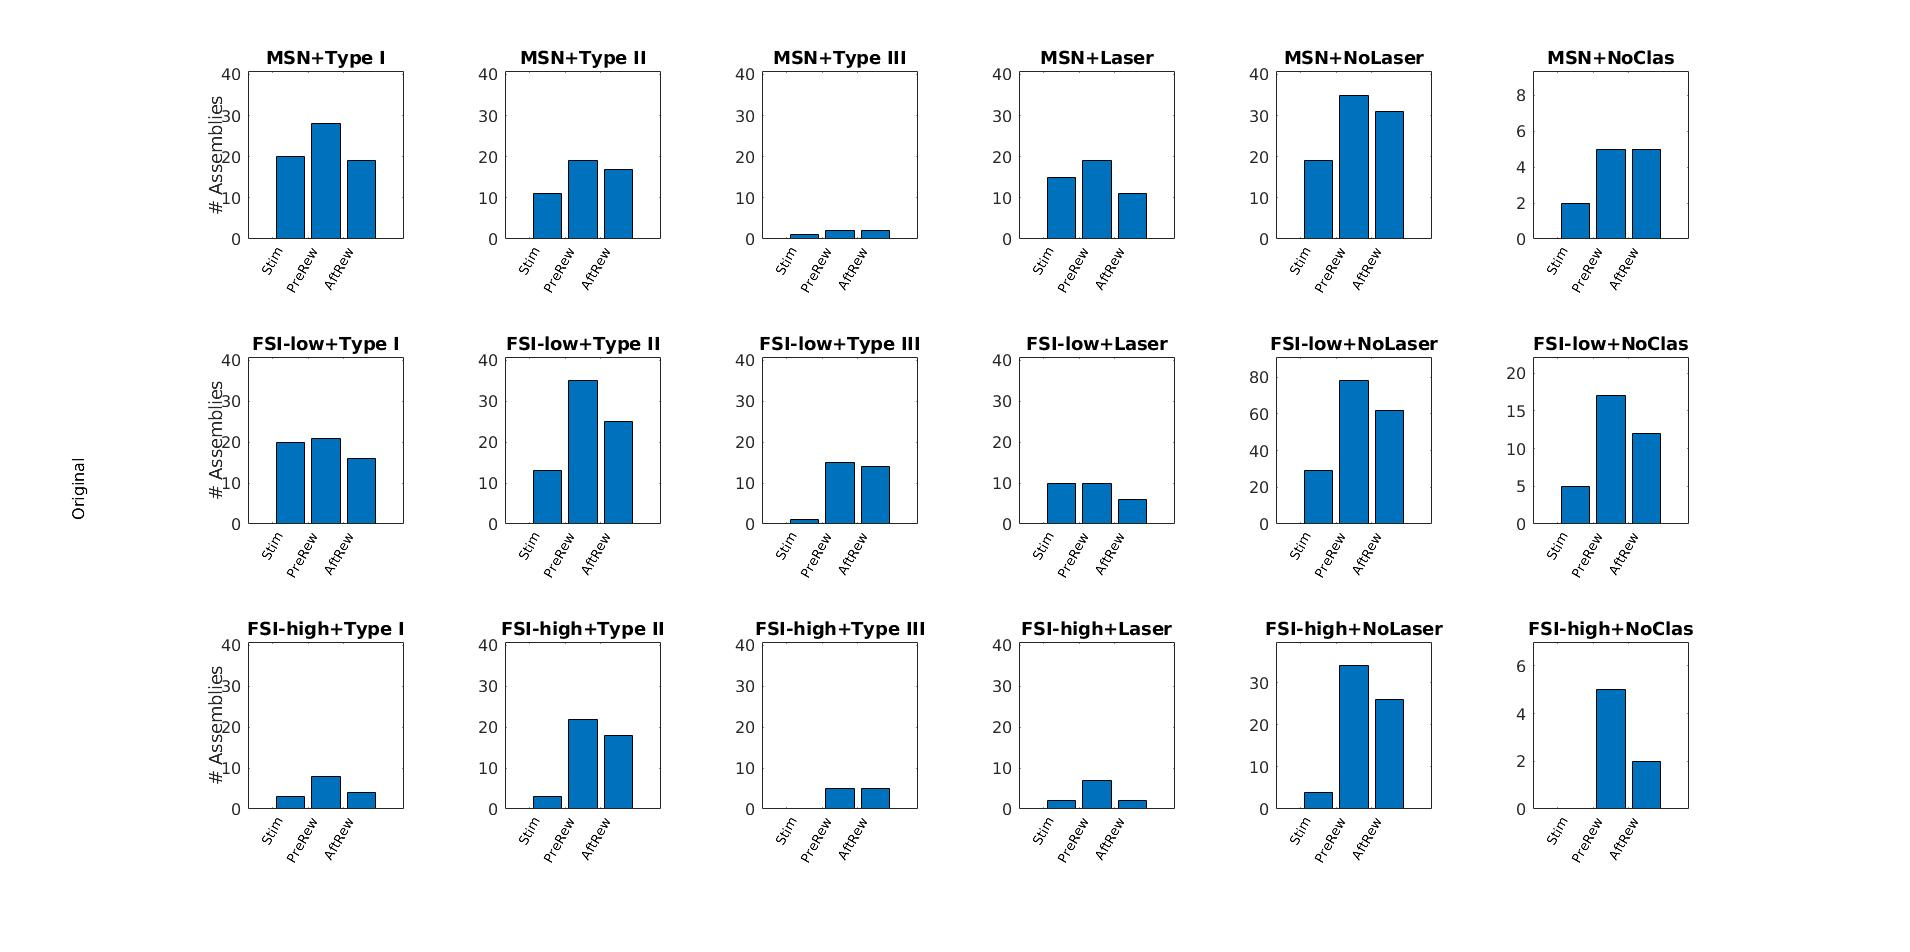
\includegraphics[scale=0.3]{figures/Original_Hit_N.jpg}
    % 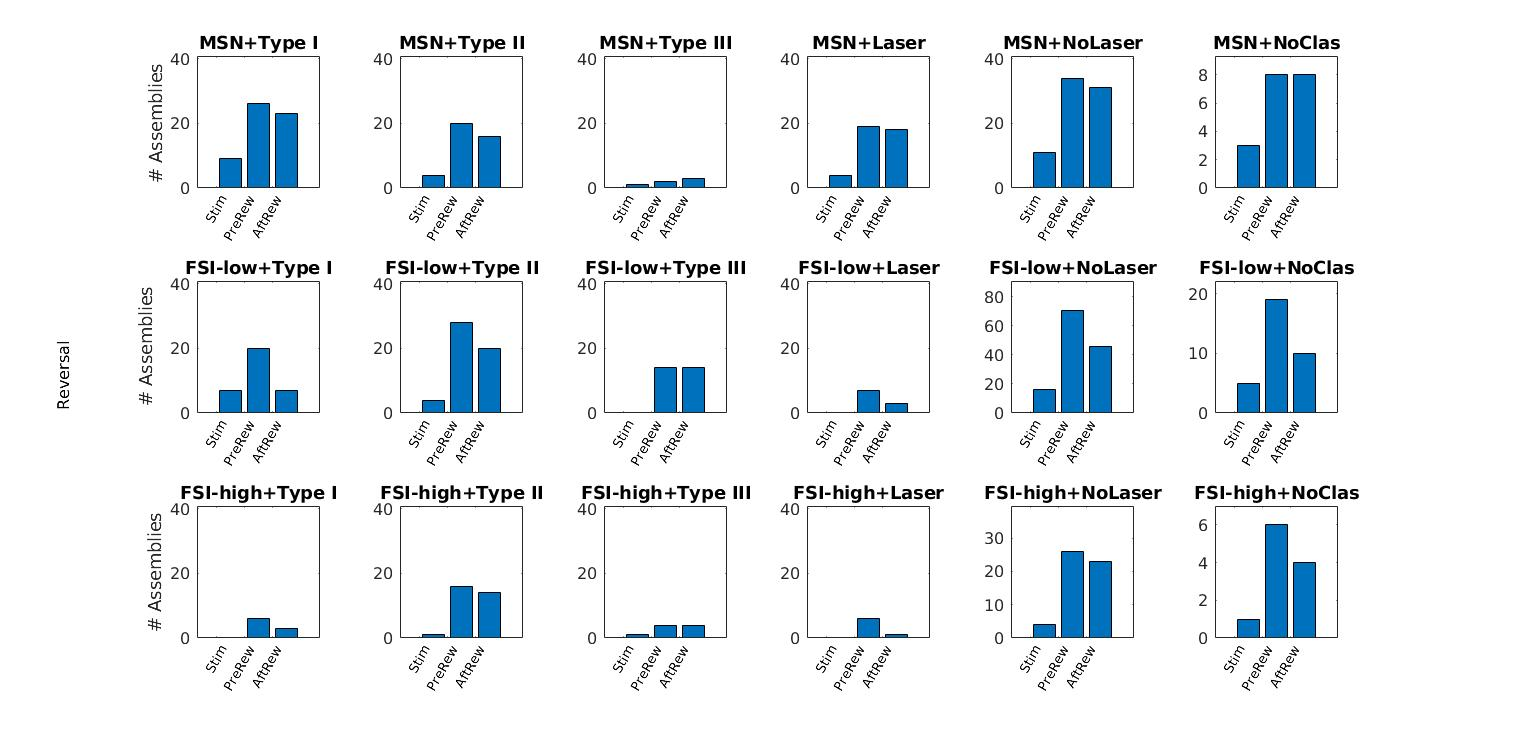
\includegraphics[scale=0.3]{figures/Reversal_Hit_N.jpg}
     %\caption{{\color{red}TO MODIFY!!!! BUT THIS IS THE PLOT}}
     %\label{fig:histo_taskrel}
 %\end{figure}
%\begin{figure}
  %  \centering
   % 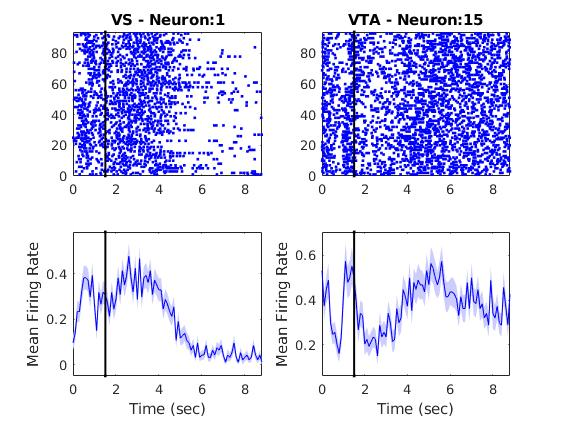
\includegraphics[scale=0.6]{figures/SingleNeus1_15Lastrev1Pru_An_4.jpg}
    %\caption{Shift in time of neuronal activity of two units in assembly. }
    %\label{fig:NeusInAsse}
%\end{figure}

%\section{Discussion}
%\section{Combination of single neuron and assemblies analysis}
%\subsection{Directionality using classification}
%\subsection{Significant task related response for typology}
To better study assemblies activation patterns, first the task relevant moments of the experiment were selected. From the mean task related activity patterns we expected to see differences among assemblies types in two experimental chapters (original and reversal). To better visualize the task related activation patterns via heat plots, hit trials (rewarded odor, mouse went for reward), correct rejection trials (unrewarded odor, mouse sat quiet), false alarm trials (unrewarded odor, mouse went for reward), were kept separated; however this separation among trials types was released in further analysis, without affecting results.
The assemblies were pruned according their significant task related activity, that was tested with Friedman's test and a non parametric version of the repeated measures Anova. We preferred to use non-parametric tests to be free from the assumption of gaussianity of the observations. Results of the two tests were consistent each other. The two relevant events of the task were the odor onset and the reward delivery, then we choose whether the assemblies showed a significant activity in three windows: Stimulus [0s, 0.5s], Pre-Reward [-0.5s, 0s], Reward [0s, 05s], the baseline was chosen in the interval [-1s, -0.5s] from the odor onset. Post-hoc analysis were performed using the Bonferroni's criterion {\color{red}check whether the criterion was Bonferroni of some other}. Almost $80\%$ of the VS-VTA assemblies showed a task related activity significant different from the baseline or from another of the windows considered. Of the significant assemblies $\%$ were composed by MSN-Type I units, $\%$ by FSI low-Type I, $\%$ by FSI high-Type I, $\%$ MSN-Type II, $\%$ by FSI low-Type II, $\%$ by FSI high-Type II, the other possible units combinations constitutes a minority and all toghether were the $\%$ {\color{red} Insert numbers of percentage}.

\section{Conclusion}
